\documentclass[a4paper,12pt]{article}
\usepackage[utf8]{inputenc}
\usepackage[spanish]{babel}
\usepackage{amsmath}
\usepackage{geometry}
\usepackage{graphicx}
\usepackage{graphics}
\usepackage[%  
    colorlinks=true,
    pdfborder={0 0 0},
    linkcolor=red
]{hyperref}
\geometry{margin=2.5cm}

\title{Informe de Trabajo Práctico 1}
\author{Aprendizaje Profundo con aplicación a Visión Artificial \\
Laura Zúñiga Osorio}
\date{\today}

\begin{document}

\maketitle

\paragraph{1. \textit{k}-nearest neighbors.} En este ejercicio, utilizamos la librería \texttt{pandas} para generar dos datasets de datos bidimensionales que les fueron asignadas distribuciones de clase particulares. En el primero, los datos de entrenamiento se forman en torno a un punto central \texttt{(n,n)} adicionando ruido aleatorio y designando la clase al entero \texttt{n}. Los datos de test se generan aumentando el ancho de la distribución en torno al punto. La clasificación se realizó implementando el método de \textit{k}-vecinos cercanos barriendo los valores de \textit{k} entre 1 y 27 en pasos de a 2.  Los puntos indicados con una \textit{x} señalan predicciones erróneas. Las distribuciones y resultados se muestran en la figura \ref{fig:ej1:knn}. Esto se repitió para una distribución de datos inspirada en la clasificación de cuadrantes del plano cartesiano, pero incluyendo una quinta clase adicional para los puntos cercanos a los ejes.

\begin{figure}[!h]
    \centering
    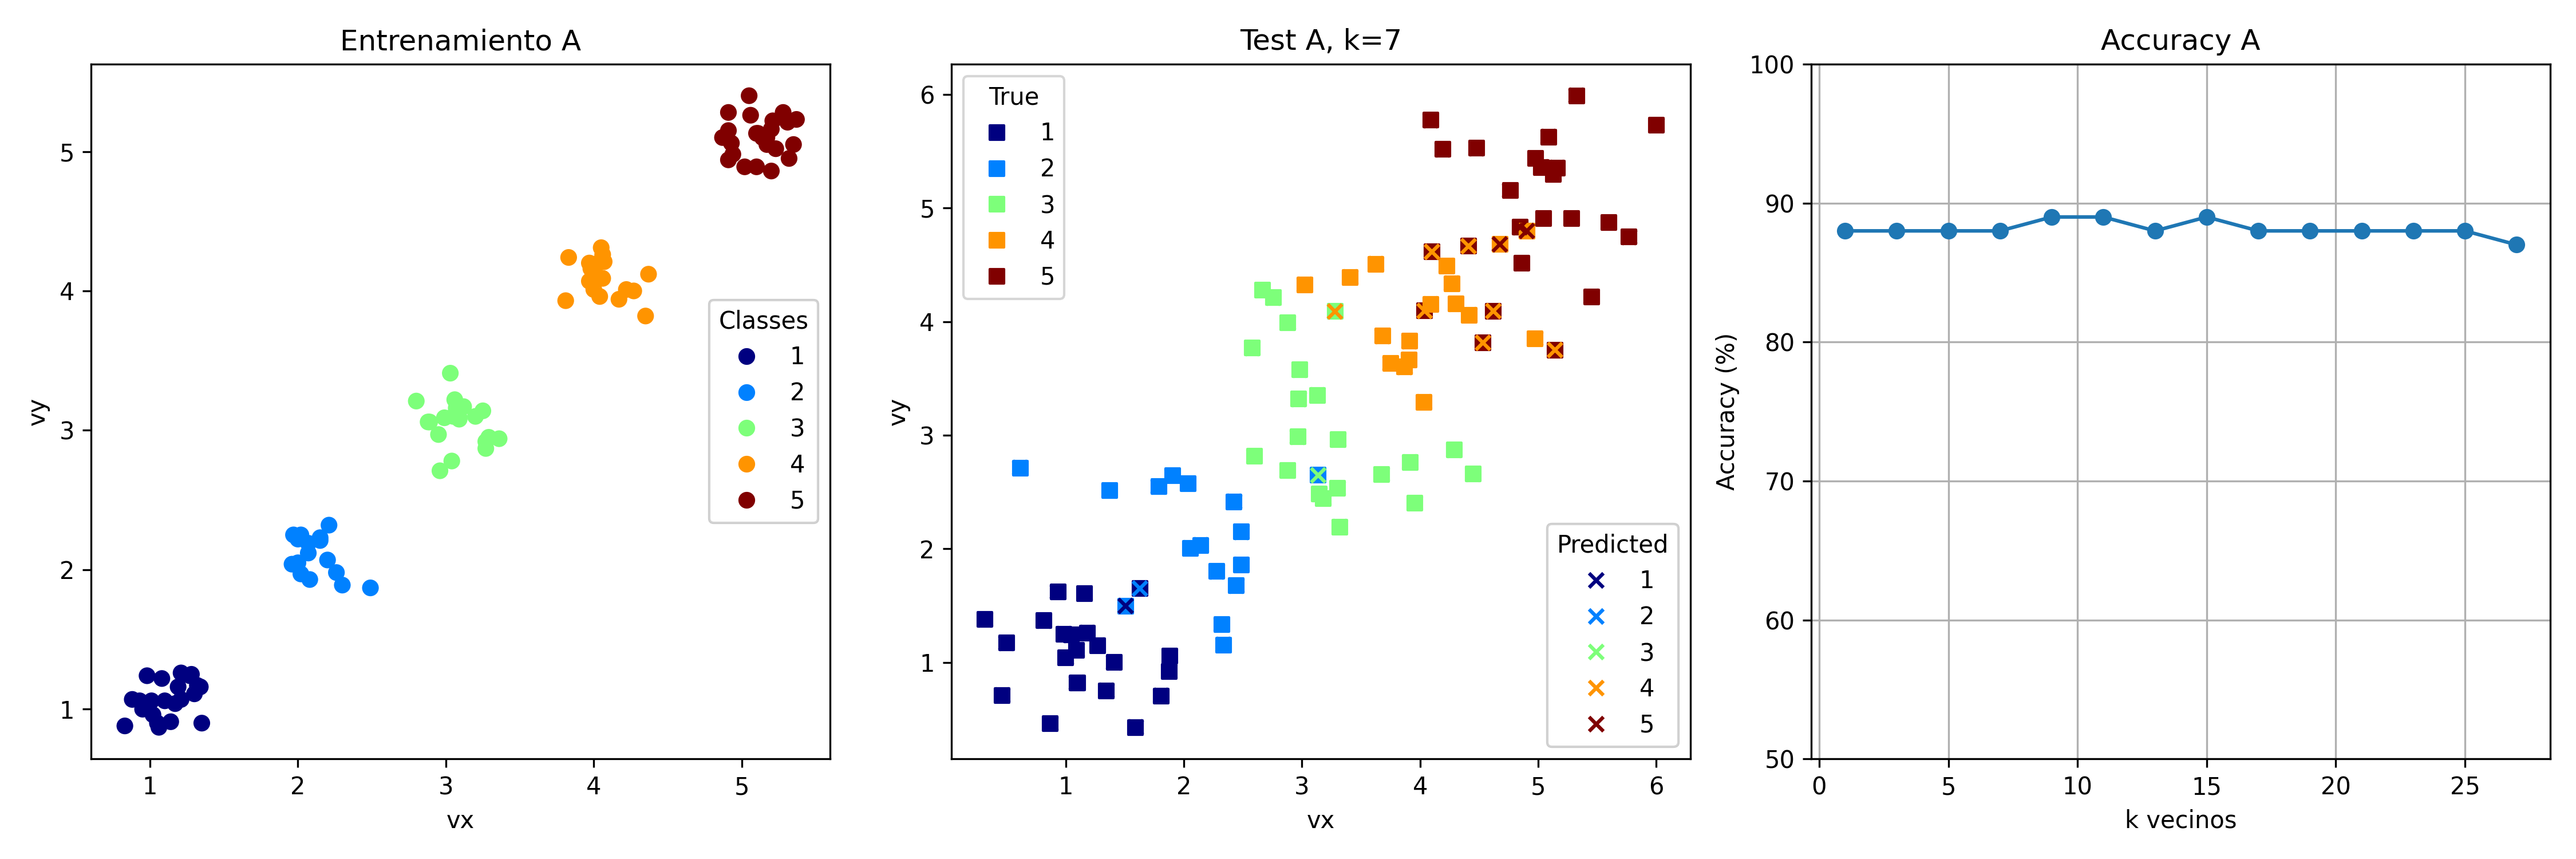
\includegraphics[width=\textwidth]{ej1_zuniga_A.png}
    \quad
    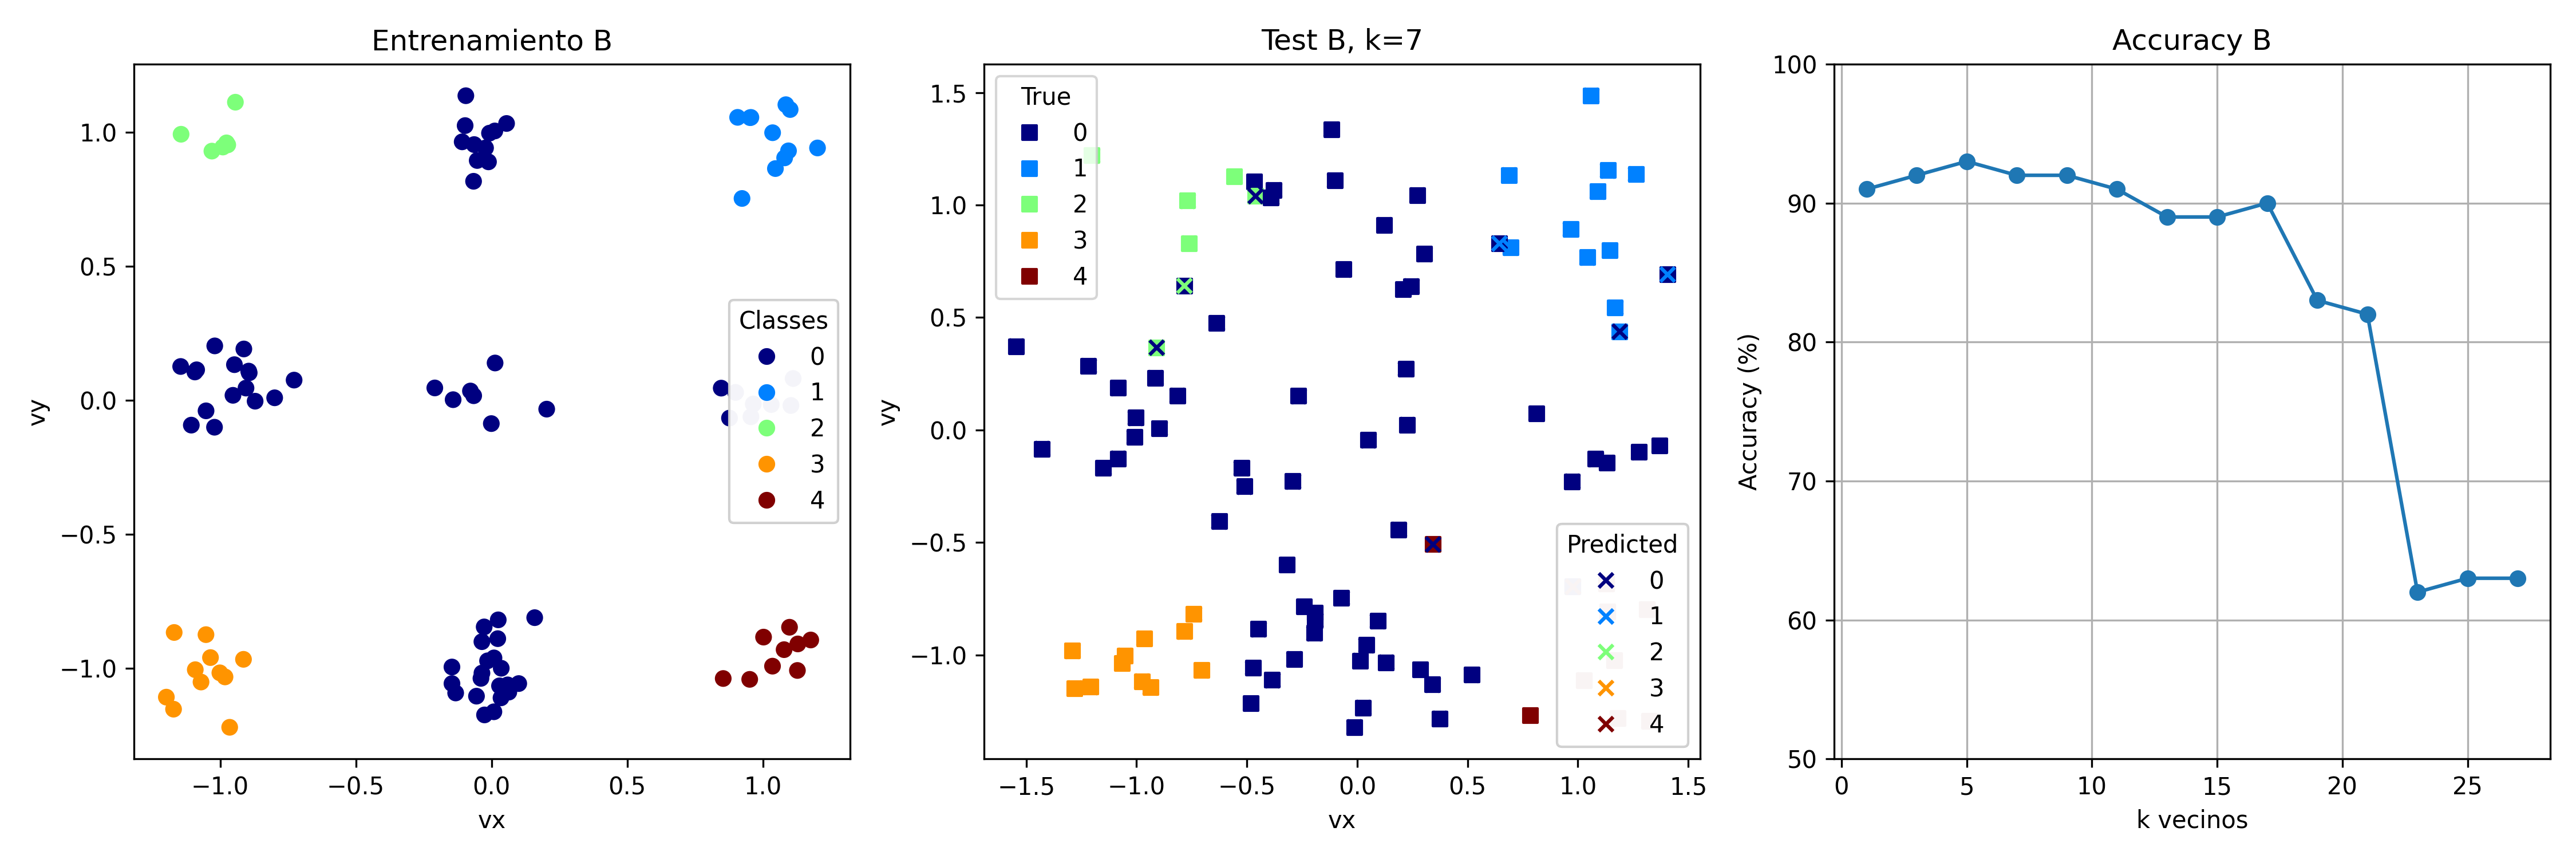
\includegraphics[width=\textwidth]{ej1_zuniga_B.png}
    \caption{Clasificación por método de \textit{k}-vecinos cercanos para dos distribuciones de datos diferentes. \label{fig:ej1:knn}}
\end{figure}

Para generar un mapa que ilustre las fronteras de decisión, se graficaron 1000 puntos del espacio con su respectiva clase predicha, como se muestra en la figura \ref{fig:ej1:decision}.

\begin{figure}[!h]
    \centering
    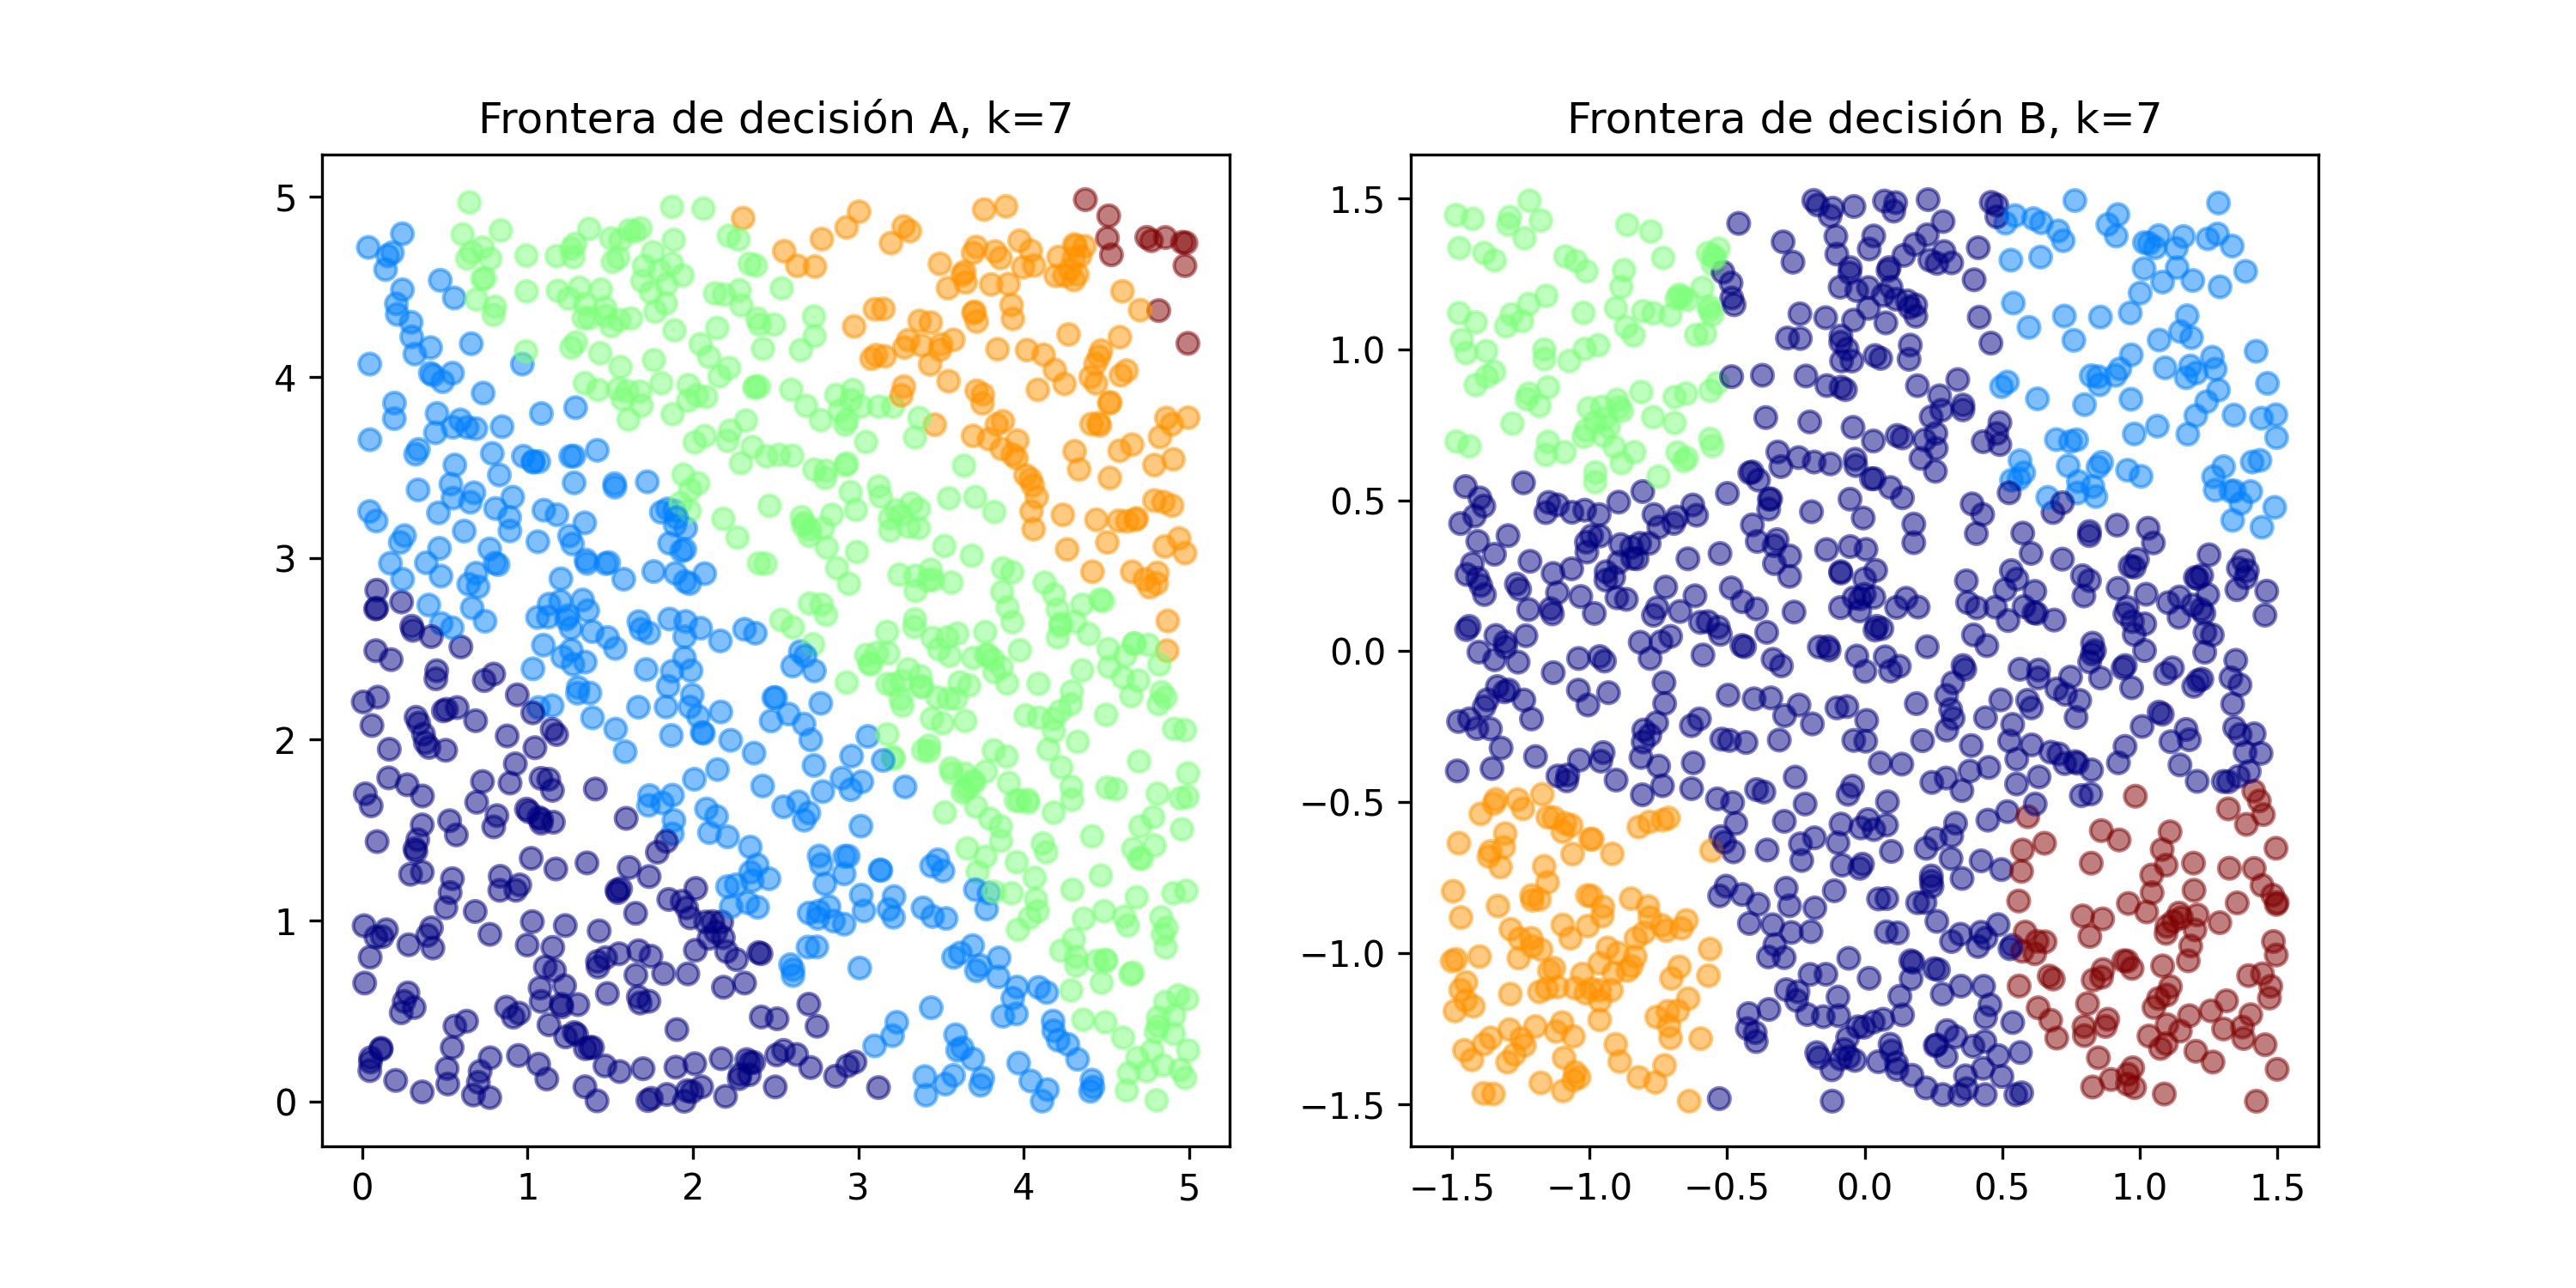
\includegraphics[width=\textwidth]{ej1_zuniga_frontera.png}    
    \caption{Zonas de decisión del clasificador para cada distribución de datos. \label{fig:ej1:decision}}
\end{figure}

\paragraph{2. \textit{k}-nearest neighborst para MNIST y CIFAR-10}. El mismo método de clasificación \textit{k}-nn se implementó con los datasets públicos MNIST (imgs. de números manuscritos del 0 al 9) y CIFAR-10 (imágenes naturales separadas en 10 clases). Para cargar los datos, se hizo uso de la librería \texttt{torchvision.datasets} y la manipulación de sus dimensiones se hizo a nivel tensorial mediante la librería \texttt{torchvision.transforms}. Los 5 primeros elementos del conjunto de test se muestran para cada uno en la figura \ref{fig:ej2:ejemplos}.

\begin{figure}[!h]
    \centering
    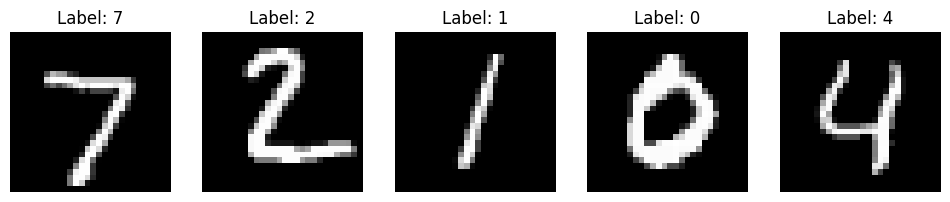
\includegraphics[width=0.8\textwidth]{ej2_mnist_examples.png}
    \quad    
    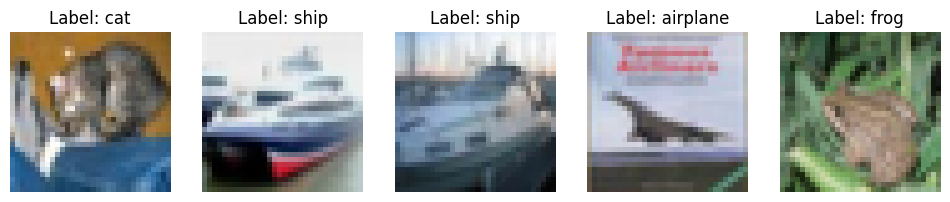
\includegraphics[width=0.8\textwidth]{ej2_cifar_examples.png}
    \caption{Ejemplos de imágenes del conjunto de test para MNIST (arriba) y CIFAR-10 (abajo). \label{fig:ej2:ejemplos}}
\end{figure}
\newpage
Los gráficos de accuracy muestreando los 20 primeros datos de cada conjunto, según el número de vecinos, se muestran en la figura \ref{fig:ej2:knn}.

\begin{figure}[!h]
    \centering
    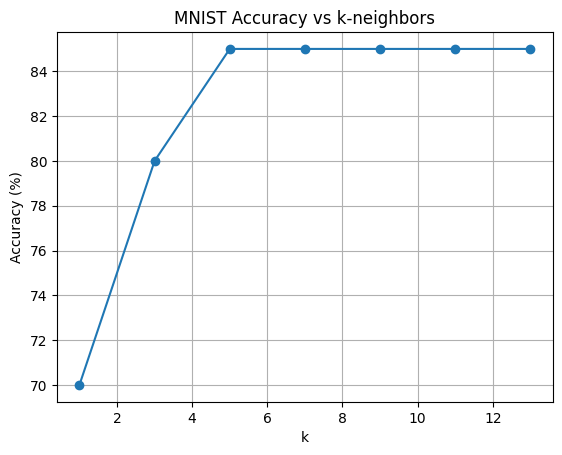
\includegraphics[width=0.45\textwidth]{ej2_mnist_knn_acc.png}
    \quad
    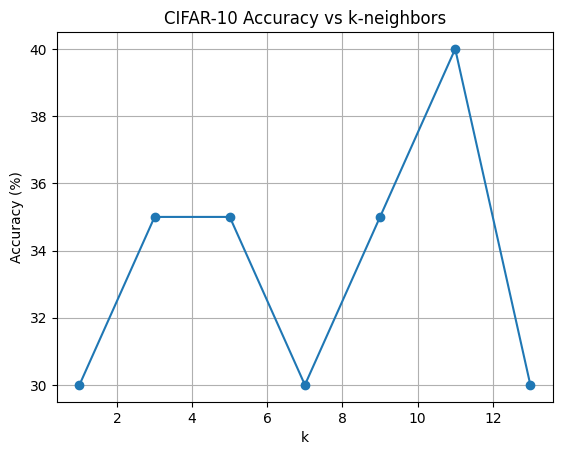
\includegraphics[width=0.45\textwidth]{ej2_cifar_knn_acc.png}
    \caption{Resultados de accuracy como función de \textit{k} para los conjuntos MNIST y CIFAR-10. \label{fig:ej2:knn}}
\end{figure}

\paragraph{3. Implementación de SVM y Softmax}
Implementamos el método de clasificación lineal SVM y SoftMax utilizando regularización L2 y el paradigma de programación orientada a objetos. Para ello, ambas clases heredan de una clase base llamada \texttt{LinearClassifier}, que provee los métodos \texttt{fit}, \texttt{predict} y el cálculo del gradiente de la función de pérdida. Además, se implementó la métrica de \textit{accuracy} para monitorear la precisión durante el entrenamiento. Evaluamos ambas implementaciones con los conjuntos de datos MNIST (figuras \ref{fig:ej3:svm}, \ref{fig:ej3:softmax}) y CIFAR-10, utilizando el método de entrenamiento mini-batch (BGD). Finalmente, comparamos la exactitud de los métodos y graficamos las curvas de pérdida y precisión para distintas épocas, tanto en entrenamiento como en evaluación, analizando cuál resulta más adecuado para cada problema.

\begin{figure}[h]
    \centering
    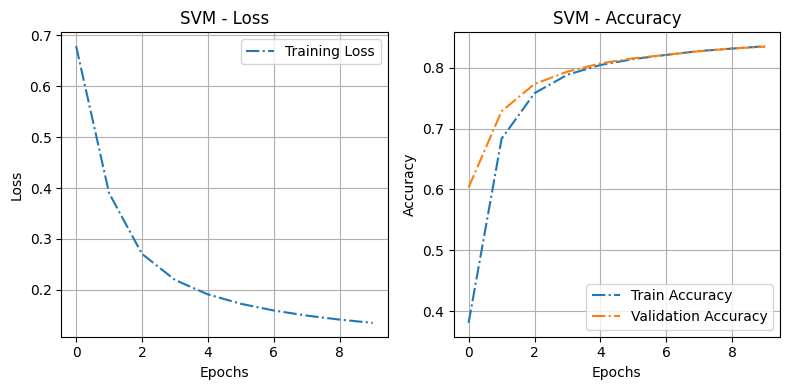
\includegraphics[width=0.8\textwidth]{ej3_svm_mnist.png}
    \caption{(MNIST) Métricas de entrenamiento para clasificador lineal. La clase heredada define la función de pérdida correspondiente al método \textit{hinge loss}, propio de Support Vector Machine. \label{fig:ej3:svm}}
\end{figure}


Los resultados después de 10 épocas del entrenamiento del conjunto CIFAR-10 se incluyen a continuación:


\noindent\textbf{SVM.} \texttt{Epoch 10: loss=0.5261, train acc=0.3488, val acc=0.3418}


\noindent\textbf{SoftMax.} \texttt{Epoch 10: loss=1.8987, train acc=0.3587, val acc=0.3450}

\begin{figure}[h]
    \centering
    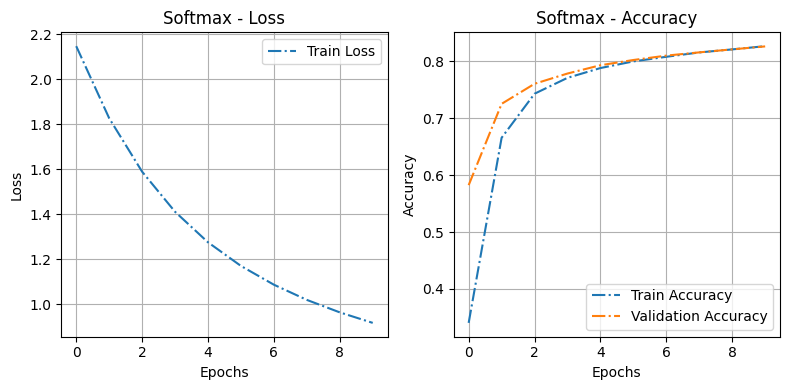
\includegraphics[width=0.8\textwidth]{ej3_softmax_mnist.png}
    \caption{(MNIST) Métricas de entrenamiento para el método SoftMax. \label{fig:ej3:softmax}}
\end{figure}

Ambos métodos obtienen mejores resultados en el conjunto MNIST después de 10 épocas. Esto puede atribuirse a la naturaleza de los datos: MNIST contiene imágenes más simples y menos variables que CIFAR-10, lo que facilita la tarea de clasificación lineal. 

\end{document}